\chapter[Documento de Arquitetura]{Documento de Arquitetura}


A finalidade do Documento de Arquitetura é definir um modelo arquitetural para ser aplicado ao desenvolvimento do sistema de anticolisões, bem como reunir todas as informações necessárias ao controle das atividades de Arquitetura, oferecendo uma visão macro dos requisitos arquiteturais e não funcionais para suportar.

\begin{enumerate}
\item \textbf{Metas e restrições da Arquitetura}

O sistema anticolisões tem por objetivo ser um sistema  que auxilia a tomada de decisões na hora da ultrapassagem . Por isso, o sistema  deverá ser seguro e sem falhas. Além disso, a arquitetura do sistema deve ser implementada de modo a permitir a evolução e manutenção do sistema. Abaixo, estão listados os requisitos que devem ser considerados para a arquitetura do sistema:

\begin{enumerate}
  \item Segurança: o sistema deve informar a distância dos carros em relação ao motorista, o sistema deve informar a possibilidade de uma ultrapassagem
  \item Disponibilidade: O sistema deverá estar disponível e ativo 24 horas por dia e 7 dias por semana.
  \item Suportabilidade: O sistema deverá funcionar em um volkswagen Gol 1.0 do ano de 2013.
\end{enumerate}

\item \textbf{Visão de Camadas}

\begin{figure}[h]
  \centering
  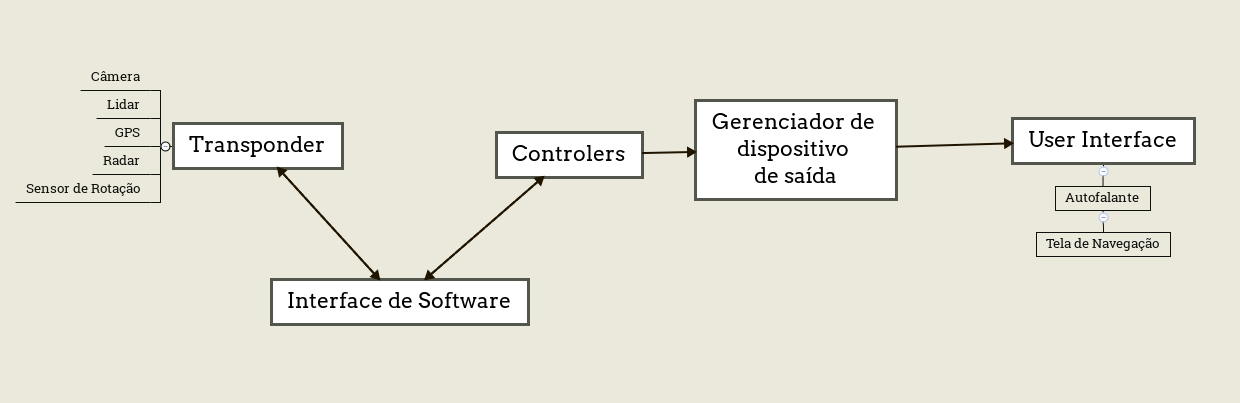
\includegraphics[width=400px, scale=1]{figuras/modelo_arquitetura}
  \caption{Modelo arquitetural do sistema}
\label{fig:modelo_arquitetura}
\end{figure}



\begin{enumerate}
  \item \textbf{Transponder:}  O transponder é responsável por receber as informações de outros dispositivos eletronicos e realizar a transmissão para o processamento do software.
  \item  \textbf{Interface de software:} Camada responsável por receber as informações que vem dos dispositivos eletronicos do sistema, e converte-los em informações que podem ser processadas pelo software
  \item \textbf{Controlers:}  Camada responsável por processar as informações que serão transmitidas dos dispositivos eletrônicos.
  \item \textbf{Gerenciador de dispositivo de saída:}  Camada responsável por fazer a conversão das informações processadas pelo sistema, para os dispositivos que utilizam recursos gráficos para o motorista.
  \item \textbf{User interface:}  Camada responsável por permitir a visualização a partir de uma interface gráfica para o motorista, lembrando que essa interface deve ser de fácil aprendizagem de uso. Devemos utilizar como referência o seguinte sistema:
\end{enumerate}

\begin{figure}[h]
  \centering
  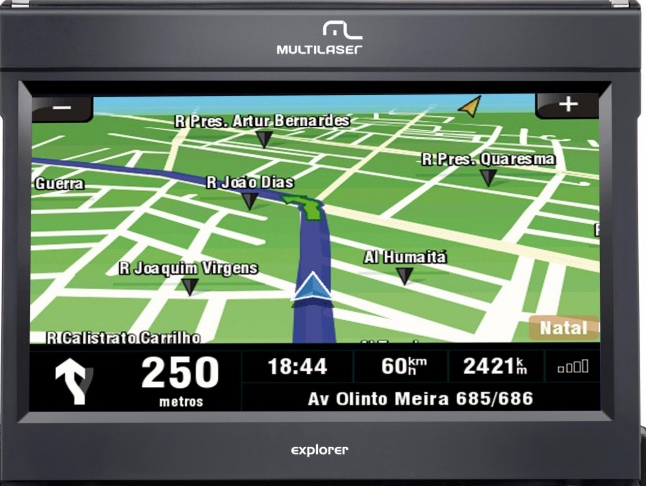
\includegraphics[width=250px, scale=1]{figuras/tela_gps}
  \caption{Modelo da tela do sistema}
\label{fig:tela_gps}
\end{figure}

\item \textbf{Visão de Implementação}
Essa seção fornece uma visão geral do modelo de implementação e da organização em termos de componentes do sistema.

\begin{enumerate}
  \item \textbf{Visão Geral}

  O diagrama de classes auxilia a visualização das classes existentes no sistema, seus atributos e seu métodos. A partir dele, também é visível o relacionamento entre as classes e também a cardinalidade entre elas. A imagem abaixo ilustra o diagrama de classe do sistema:

  \item \textbf{Diagrama de Classe }
  \begin{figure}[h]
    \centering
    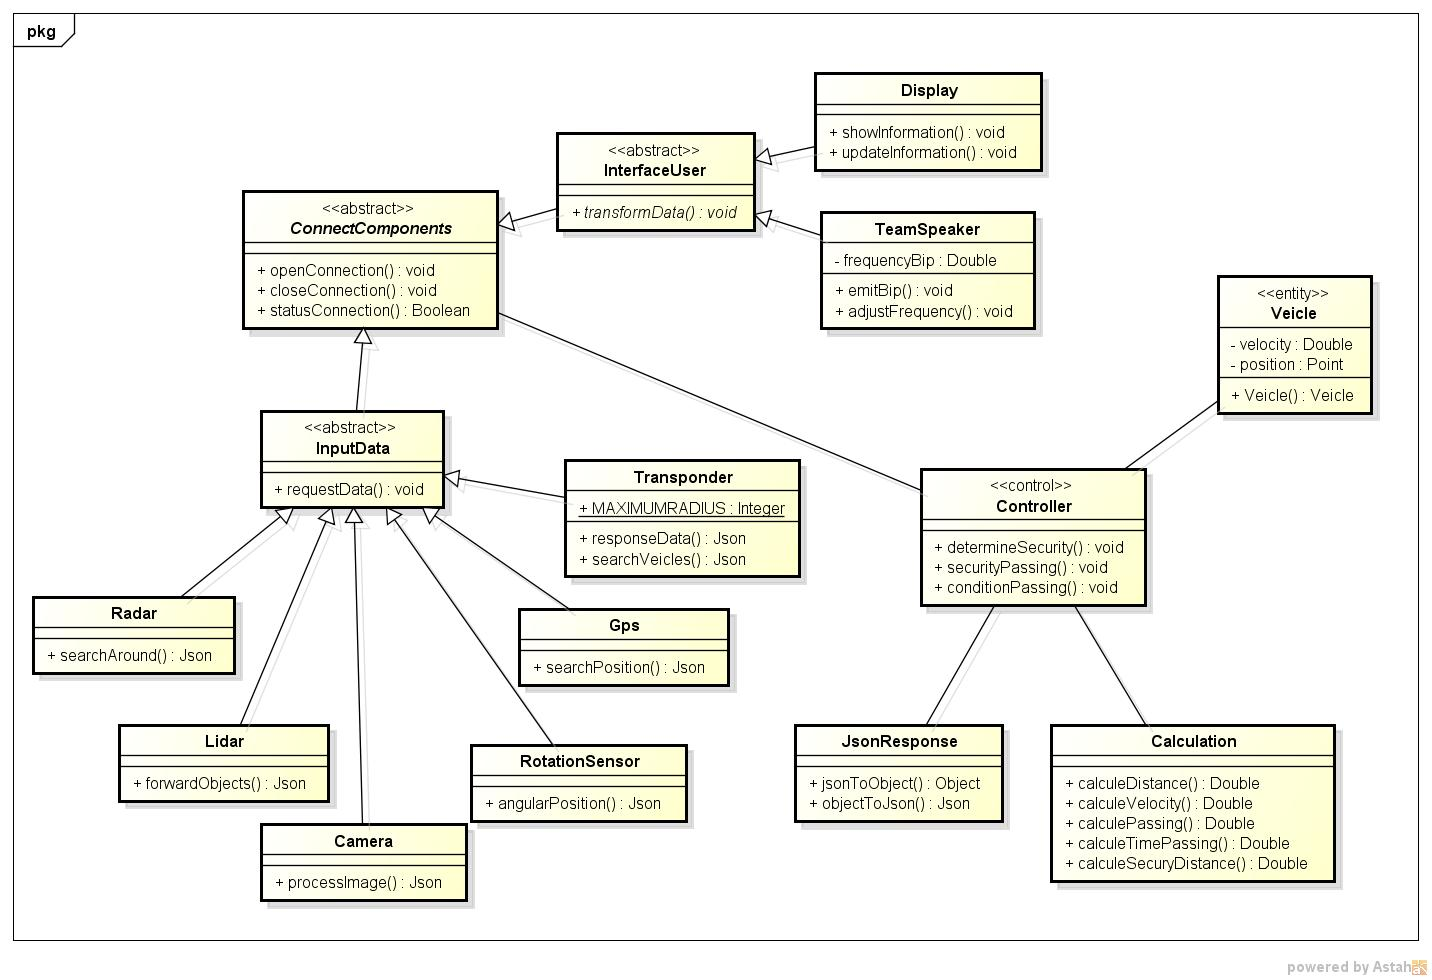
\includegraphics[width=450px, scale=1]{figuras/diagrama_classes}
    \caption{Diagrama de Classes do sistema}
  \label{fig:diagrama_classes}
  \end{figure}

\end{enumerate}


\end{enumerate}
